\documentclass[12pt]{article}
\usepackage{tikz}
\usetikzlibrary{arrows.meta, shapes, calc, backgrounds, positioning, patterns, decorations.markings, decorations.pathmorphing, decorations.pathreplacing, decorations.text, fit, matrix, shadings}
\usepackage{xcolor}
\usepackage{graphicx}

\begin{document}

\section*{TeXpresso TikZ Support Test}

\subsection*{Phase 0: Dash Patterns (long pattern > 4 elements)}

\begin{tikzpicture}
  % 5 element dash pattern
  \draw[dash pattern=on 4pt off 2pt on 8pt off 3pt on 12pt off 4pt] (0,0) -- (8,0);
  \draw[dash pattern=on 5pt off 3pt on 7pt off 4pt on 9pt off 2pt on 3pt off 1pt] (0,-0.5) -- (8,-0.5);
\end{tikzpicture}

\subsection*{Phase 1: Text Nodes}

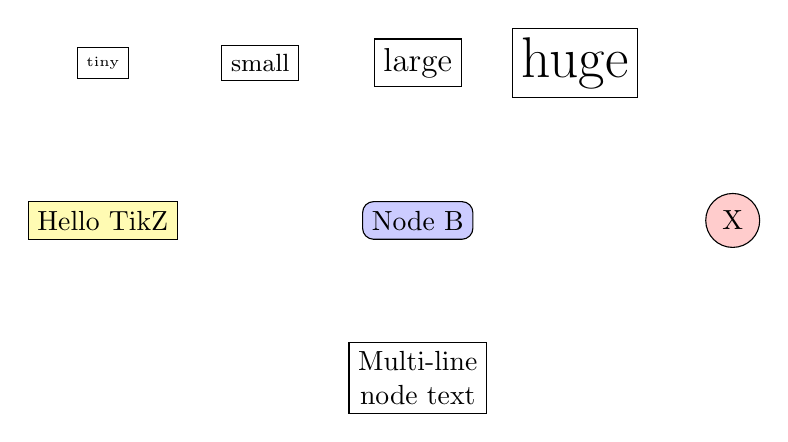
\begin{tikzpicture}
  % basic node labels
  \node[draw, fill=yellow!30] at (0,0) {Hello TikZ};
  \node[draw, fill=blue!20, rounded corners] at (4,0) {Node B};
  \node[draw, circle, fill=red!20] at (8,0) {X};

  % different font size nodes
  \node[draw] at (0,2) {\tiny tiny};
  \node[draw] at (2,2) {\small small};
  \node[draw] at (4,2) {\large large};
  \node[draw] at (6,2) {\huge huge};

  % multi-line node (align)
  \node[draw, align=center] at (4,-2) {Multi-line\\node text};
\end{tikzpicture}

\subsection*{Phase 1: Basic Paths (supported)}

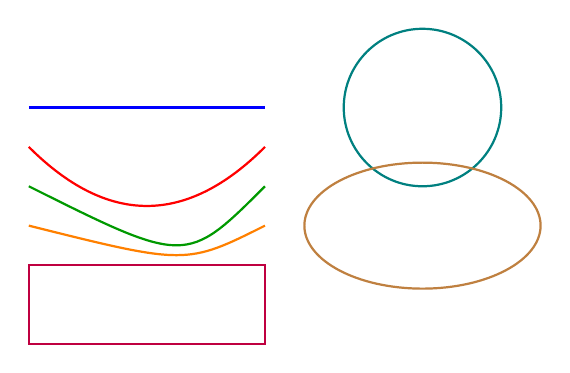
\begin{tikzpicture}
  % lines
  \draw[blue, thick] (0,0) -- (3,0);
  % curves (c, v, y)
  \draw[red, thick] (0,-0.5) .. controls (1,-1.5) and (2,-1.5) .. (3,-0.5);
  \draw[green!60!black, thick] (0,-1) .. controls (2,-2) .. (3,-1);
  \draw[orange, thick] (0,-1.5) .. controls (2,-2) and (2,-2) .. (3,-1.5);
  % rectangle
  \draw[purple, thick] (0,-2) rectangle (3,-3);
  % circle and ellipse
  \draw[teal, thick] (5,0) circle (1);
  \draw[brown, thick] (5,-1.5) ellipse (1.5 and 0.8);
\end{tikzpicture}

\subsection*{Phase 1: Fill and Stroke}

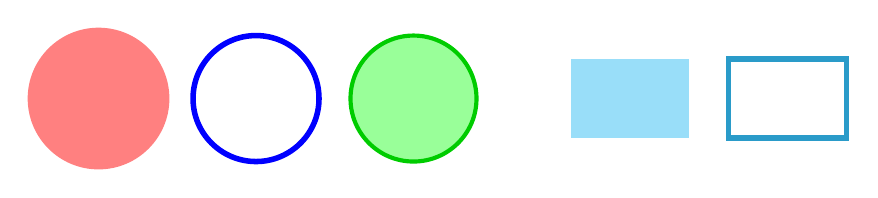
\begin{tikzpicture}
  % fill only
  \fill[red!50] (0,0) circle (0.9);
  % draw only
  \draw[blue, line width=2pt] (2,0) circle (0.8);
  % fill + draw
  \filldraw[fill=green!40, draw=green!80!black, line width=1.5pt] (4,0) circle (0.8);

  % rectangles
  \fill[cyan!40] (6,-0.5) rectangle (7.5,0.5);
  \draw[cyan!80!black, line width=2pt] (8,-0.5) rectangle (9.5,0.5);
\end{tikzpicture}

\subsection*{Phase 1: Line Types (width, join, cap, dash)}

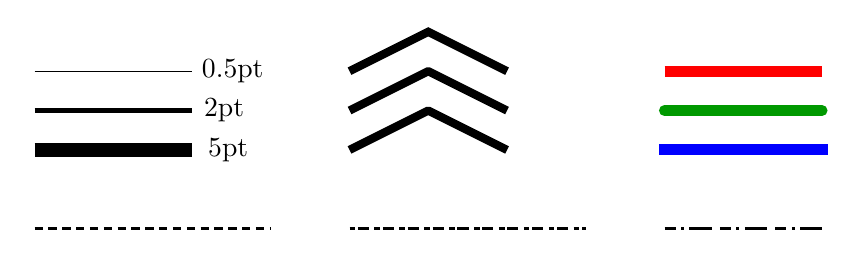
\begin{tikzpicture}
  % line width
  \draw[line width=0.5pt] (0,0) -- (2,0) node[right] {0.5pt};
  \draw[line width=2pt] (0,-0.5) -- (2,-0.5) node[right] {2pt};
  \draw[line width=5pt] (0,-1) -- (2,-1) node[right] {5pt};

  % line join
  \draw[line width=3pt, line join=miter] (4,0) -- (5,0.5) -- (6,0);
  \draw[line width=3pt, line join=round] (4,-0.5) -- (5,0) -- (6,-0.5);
  \draw[line width=3pt, line join=bevel] (4,-1) -- (5,-0.5) -- (6,-1);

  % line cap
  \draw[line width=4pt, line cap=butt, red] (8,0) -- (10,0);
  \draw[line width=4pt, line cap=round, green!60!black] (8,-0.5) -- (10,-0.5);
  \draw[line width=4pt, line cap=rect, blue] (8,-1) -- (10,-1);

  % dash patterns
  \draw[line width=1pt, dash pattern=on 3pt off 2pt] (0,-2) -- (3,-2);
  \draw[line width=1pt, dash pattern=on 2pt off 1pt on 4pt off 2pt] (4,-2) -- (7,-2);
  \draw[line width=1pt, dash pattern=on 4pt off 2pt on 1pt off 2pt on 8pt off 3pt] (8,-2) -- (10,-2);
\end{tikzpicture}

\subsection*{Phase 1: Color Modes}

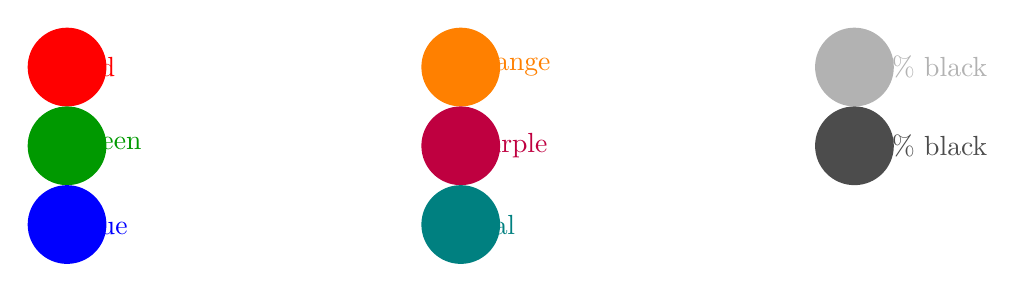
\begin{tikzpicture}
  % named colors
  \fill[red] (0,0) circle (0.5) node[right] {red};
  \fill[green!60!black] (0,-1) circle (0.5) node[right] {green};
  \fill[blue] (0,-2) circle (0.5) node[right] {blue};

  % mixed colors
  \fill[orange] (5,0) circle (0.5) node[right] {orange};
  \fill[purple] (5,-1) circle (0.5) node[right] {purple};
  \fill[teal] (5,-2) circle (0.5) node[right] {teal};

  % gray
  \fill[black!30] (10,0) circle (0.5) node[right] {30\% black};
  \fill[black!70] (10,-1) circle (0.5) node[right] {70\% black};
\end{tikzpicture}

\subsection*{Phase 1: Graphics State (q/Q, cm, W)}

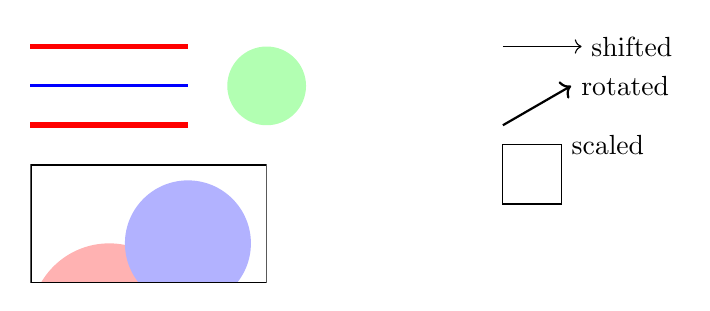
\begin{tikzpicture}
  % q/Q: save/restore state
  \begin{scope}[red, line width=2pt]
    \draw (0,0) -- (2,0);
    \begin{scope}[blue, line width=1pt]
      \draw (0,-0.5) -- (2,-0.5);
      \fill[green!30] (3,-0.5) circle (0.5);
    \end{scope}
    \draw (0,-1) -- (2,-1);
  \end{scope}

  % cm: transform
  \begin{scope}[shift={(6,0)}]
    \draw[->] (0,0) -- (1,0) node[right] {shifted};
  \end{scope}

  % rotation
  \begin{scope}[shift={(6,-1)}, rotate=30]
    \draw[->, thick] (0,0) -- (1,0) node[right] {rotated};
  \end{scope}

  % scale
  \begin{scope}[shift={(6,-2)}, scale=1.5]
    \draw (0,0) rectangle (0.5,0.5) node[right] {scaled};
  \end{scope}

  % clip (W)
  \begin{scope}
    \clip (0,-3) rectangle (3,-1.5);
    \fill[red!30] (1,-3.5) circle (1);
    \fill[blue!30] (2,-2.5) circle (0.8);
    \draw[thick] (0,-3) rectangle (3,-1.5);
  \end{scope}
\end{tikzpicture}

\subsection*{Phase 1: Path Operators (m, l, c, v, y, h, re)}

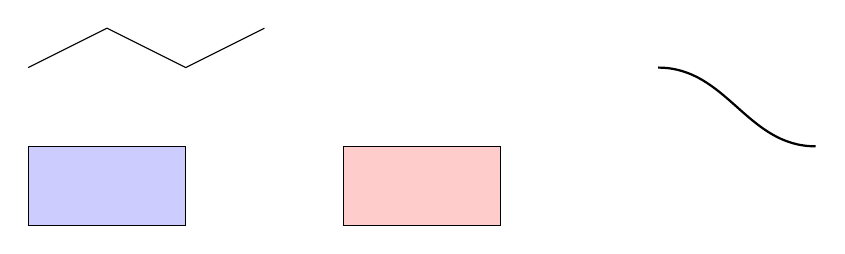
\begin{tikzpicture}
  % m (moveto) + l (lineto): \draw
  \draw (0,0) -- (1,0.5) -- (2,0) -- (3,0.5);
  % h (closepath): -- cycle
  \draw[fill=blue!20] (0,-1) -- (2,-1) -- (2,-2) -- (0,-2) -- cycle;
  % re (rectangle)
  \draw[fill=red!20] (4,-1) rectangle (6,-2);
  % combined: v + y (curves)
  \draw[thick] (8,0) to[out=0, in=180] (10,-1);
\end{tikzpicture}

\subsection*{Phase 4: Alpha / Transparency}

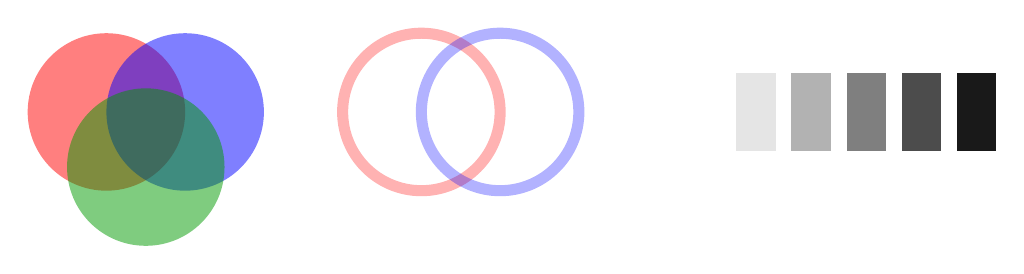
\begin{tikzpicture}
  % fill opacity
  \fill[red, fill opacity=0.5] (0,0) circle (1);
  \fill[blue, fill opacity=0.5] (1,0) circle (1);
  \fill[green!60!black, fill opacity=0.5] (0.5,-0.7) circle (1);

  % draw opacity
  \draw[red, line width=4pt, draw opacity=0.3] (4,0) circle (1);
  \draw[blue, line width=4pt, draw opacity=0.3] (5,0) circle (1);

  % different opacity levels
  \foreach \i/\op in {0/0.1, 0.7/0.3, 1.4/0.5, 2.1/0.7, 2.8/0.9} {
      \fill[black, fill opacity=\op] (\i+8,-0.5) rectangle (\i+8.5,0.5);
    }
\end{tikzpicture}

\subsection*{Phase 5: Marked Content (BMC/BDC/EMC - no-op) and Decorations}

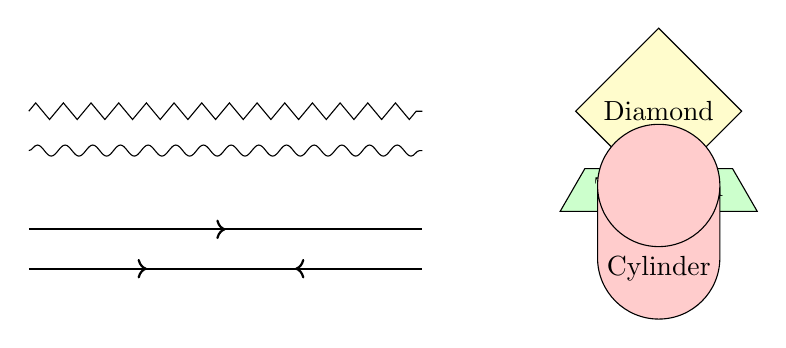
\begin{tikzpicture}
  % BMC/BDC/EMC test: layers (tikz internal)
  % decorations.markings (pathmorphing may also use marked content)
  \draw[decorate, decoration={zigzag, amplitude=3pt}] (0,0) -- (5,0);
  \draw[decorate, decoration={snake, amplitude=2pt}] (0,-0.5) -- (5,-0.5);

  % decorations.markings
  \draw[postaction={decorate, decoration={markings, mark=at position 0.5 with {\arrow{>}}}},
    thick] (0,-1.5) -- (5,-1.5);
  \draw[postaction={decorate, decoration={markings, mark=at position 0.3 with {\arrow{>}},
            mark=at position 0.7 with {\arrow{<}}}},
    thick] (0,-2) -- (5,-2);

  % shapes
  \node[draw, diamond, fill=yellow!20] at (8,0) {Diamond};
  \node[draw, trapezium, fill=green!20] at (8,-1) {Trapezium};
  \node[draw, cylinder, shape border rotate=90, fill=red!20] at (8,-2) {Cylinder};
\end{tikzpicture}

\subsection*{Combined Test: Complex Graphics with Text}

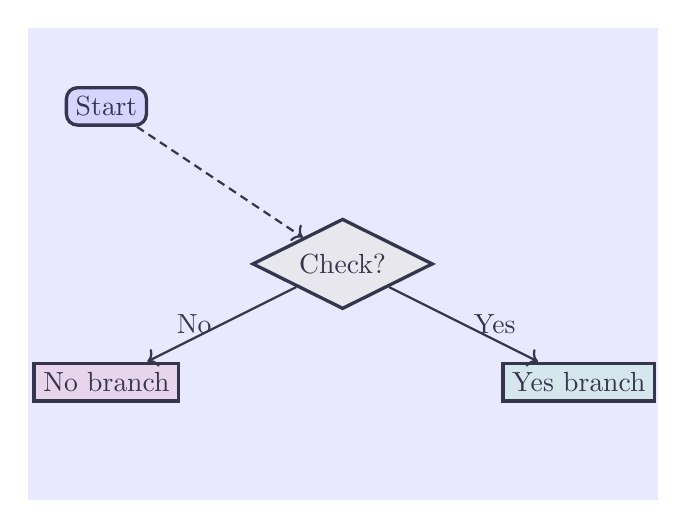
\begin{tikzpicture}
  % flow chart
  \node[draw, rounded corners, fill=blue!10, line width=1.2pt]
  (start) at (0,0) {Start};
  \node[draw, diamond, fill=yellow!10, aspect=2, line width=1.2pt]
  (check) at (3,-2) {Check?};
  \node[draw, fill=green!10, line width=1.2pt]
  (yes) at (6,-3.5) {Yes branch};
  \node[draw, fill=red!10, line width=1.2pt]
  (no) at (0,-3.5) {No branch};

  \draw[->, thick, dash pattern=on 3pt off 2pt] (start) -- (check);
  \draw[->, thick] (check) -- (yes) node[midway, right] {Yes};
  \draw[->, thick] (check) -- (no) node[midway, left] {No};

  % transparency overlay
  \fill[blue!30, fill opacity=0.3] (-1,-5) rectangle (7,1);
\end{tikzpicture}

\subsection*{Combined Test: Coordinate System and Labels}

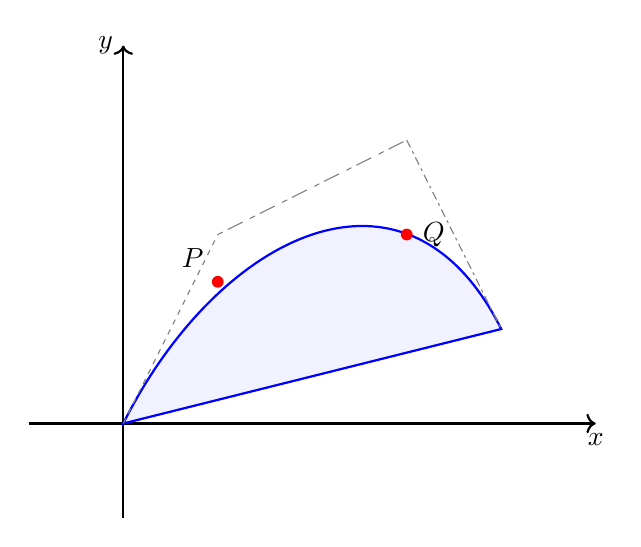
\begin{tikzpicture}[scale=1.2]
  % coordinate axes
  \draw[->, thick] (-1,0) -- (5,0) node[below] {$x$};
  \draw[->, thick] (0,-1) -- (0,4) node[left] {$y$};

  % curve
  \draw[blue, thick, fill=blue!10, fill opacity=0.5]
  (0,0) .. controls (1,2) and (3,3) .. (4,1) -- cycle;

  % label points
  \node[circle, fill=red, inner sep=1.5pt, label=above left:{$P$}] at (1,1.5) {};
  \node[circle, fill=red, inner sep=1.5pt, label=right:{$Q$}] at (3,2) {};

  % dashed control lines
  \draw[dashed, dash pattern=on 2pt off 2pt, gray] (0,0) -- (1,2);
  \draw[dashed, dash pattern=on 2pt off 2pt on 6pt off 3pt, gray] (1,2) -- (3,3);
  \draw[dashed, dash pattern=on 3pt off 1.5pt on 1pt off 1.5pt, gray] (3,3) -- (4,1);
\end{tikzpicture}

\subsection*{Phase 6: Arrows and Advanced Node Placement}

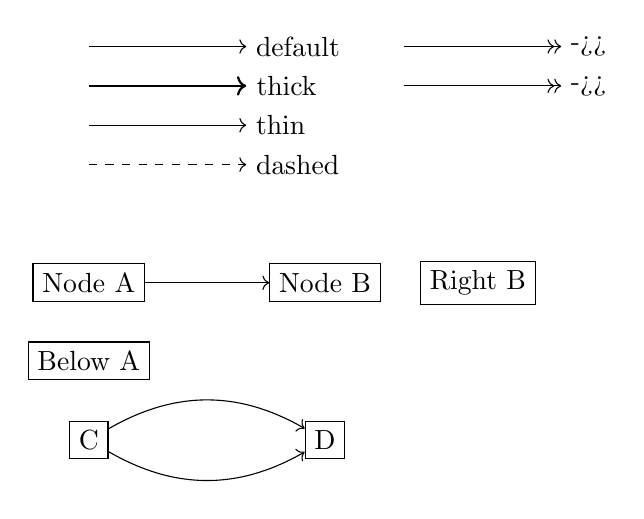
\begin{tikzpicture}
  % various arrow tips
  \draw[->] (0,0) -- (2,0) node[right] {default};
  \draw[->, thick] (0,-0.5) -- (2,-0.5) node[right] {thick};
  \draw[->, thin] (0,-1) -- (2,-1) node[right] {thin};
  \draw[->, dashed] (0,-1.5) -- (2,-1.5) node[right] {dashed};

  % different arrow styles
  \draw[->>] (4,0) -- (6,0) node[right] {->>};
  \draw[->>] (4,-0.5) -- (6,-0.5) node[right] {->>};

  % node positioning with named anchors
  \node[draw] (A) at (0,-3) {Node A};
  \node[draw] (B) at (3,-3) {Node B};
  \draw[->] (A) -- (B);
  \node[draw, below=0.5cm of A] {Below A};
  \node[draw, right=0.5cm of B] {Right B};

  % curved arrows
  \node[draw] (C) at (0,-5) {C};
  \node[draw] (D) at (3,-5) {D};
  \draw[->, bend left] (C) to (D);
  \draw[->, bend right] (C) to (D);
\end{tikzpicture}

\subsection*{Phase 7: Resizebox / Scaling}

% Test resizebox: shrink a tikzpicture to 40% of text width
{
  \centering
  \resizebox{0.4\textwidth}{!}{%
    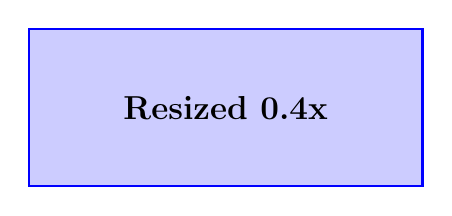
\begin{tikzpicture}
      \fill[blue!20] (0,0) rectangle (5,2);
      \draw[blue, thick] (0,0) rectangle (5,2);
      \node[font=\large\bfseries] at (2.5,1) {Resized 0.4x};
    \end{tikzpicture}%
  }
}

\subsection*{Phase 8: Complex Path Operations}

\begin{tikzpicture}
  % arc
  \draw[thick] (0,0) arc (0:180:2);
  \draw[thick, dashed] (4,0) arc (0:-180:2);

  % grid
  \draw[gray, very thin] (0,-2) grid (3,-0.5);
  \draw[blue] (0,-2) rectangle (3,-0.5);

  % parabola
  \draw[thick] (5,0) parabola bend (6,2) (7,0);
  \draw[thick, red] (5,-1) parabola (7,-0.5);

  % sin / cos (via plot coordinates)
  \draw[blue, thick] plot coordinates {(0,-2) (0.5,-1.5) (1,-1) (1.5,-0.5) (2,0)};

  % to with various options
  \draw (8,0) to[out=45, in=135] (10,0);
  \draw (8,-0.5) to[bend left] (10,-0.5);
  \draw (8,-1) to[out=-45, in=-135, looseness=2] (10,-1);
\end{tikzpicture}

\subsection*{Phase 9: Matrix and Fit}

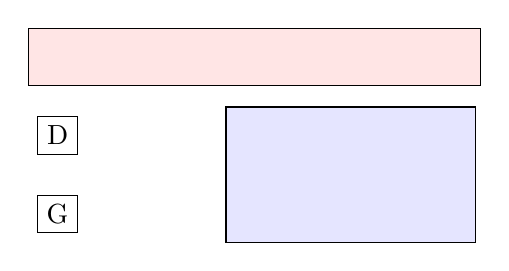
\begin{tikzpicture}
  % matrix
  % grid of named nodes (avoids \& issues with matrix)
  \node[draw] (m11) at (0,0) {A};
  \node[draw] (m12) at (2.5,0) {B};
  \node[draw] (m13) at (5,0) {C};
  \node[draw] (m21) at (0,-1) {D};
  \node[draw] (m22) at (2.5,-1) {E};
  \node[draw] (m23) at (5,-1) {F};
  \node[draw] (m31) at (0,-2) {G};
  \node[draw] (m32) at (2.5,-2) {H};
  \node[draw] (m33) at (5,-2) {I};
  \node[draw, fit=(m11)(m13), fill=red!10] {};
  \node[draw, fit=(m22)(m33), fill=blue!10] {};
\end{tikzpicture}

\subsection*{Phase 10: Foreach and Calculations}

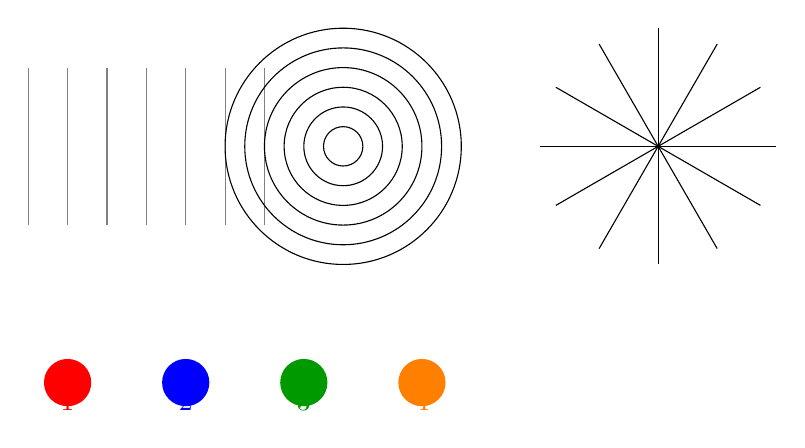
\begin{tikzpicture}
  % foreach loop
  \foreach \x in {0,0.5,...,3} {
      \draw[gray] (\x,0) -- (\x,2);
    }

  % concentric circles
  \foreach \r in {0.25,0.5,0.75,1,1.25,1.5} {
      \draw (4,1) circle (\r);
    }

  % radial lines using foreach
  \foreach \angle in {0,30,...,330} {
      \draw (8,1) -- ++(\angle:1.5);
    }

  % labeled points with foreach
  \foreach \x/\c in {1/red, 2/blue, 3/green!60!black, 4/orange} {
      \fill[\c] (\x*1.5-1,-2) circle (0.3) node[below] {\x};
    }
\end{tikzpicture}

\subsection*{Phase 11: Edge Cases and Advanced Features}

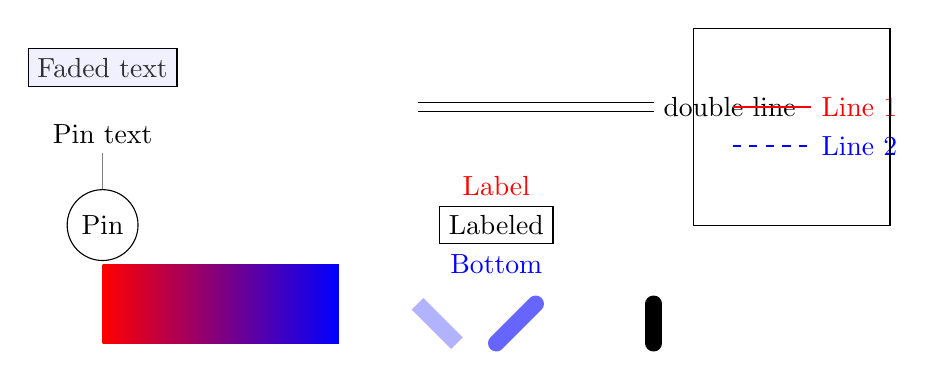
\begin{tikzpicture}
  % opacity on text
  \node[draw, fill=blue!20, fill opacity=0.3, text opacity=0.8] at (0,0)
  {Faded text};

  % double line
  \draw[double, double distance=3pt] (4,-0.5) -- (7,-0.5)
  node[right] {double line};

  % pin
  \node[circle, draw, pin=above:Pin text] at (0,-2) {Pin};

  % label with distance
  \node[draw, label={[red]90:Label}, label={[blue]-90:Bottom}] at (5,-2) {Labeled};

  % shading (basic)
  \shade[left color=red, right color=blue] (0,-3.5) rectangle (3,-2.5);

  % precision line join/cap cases
  \draw[line width=6pt, blue!30] (4,-3) -- (4.5,-3.5);
  \draw[line width=6pt, line cap=round, blue!60] (5.5,-3) -- (5,-3.5);
  \draw[line width=6pt, line cap=round] (7,-3) -- (7,-3.5);

  % legend style via scope
  \draw[red, thick] (8,-0.5) -- (9,-0.5) node[right] {Line 1};
  \draw[blue, thick, dashed] (8,-1) -- (9,-1) node[right] {Line 2};
  \draw (7.5,-2) rectangle (10,0.5);
\end{tikzpicture}

\subsection*{Phase 12: Shading Variants}

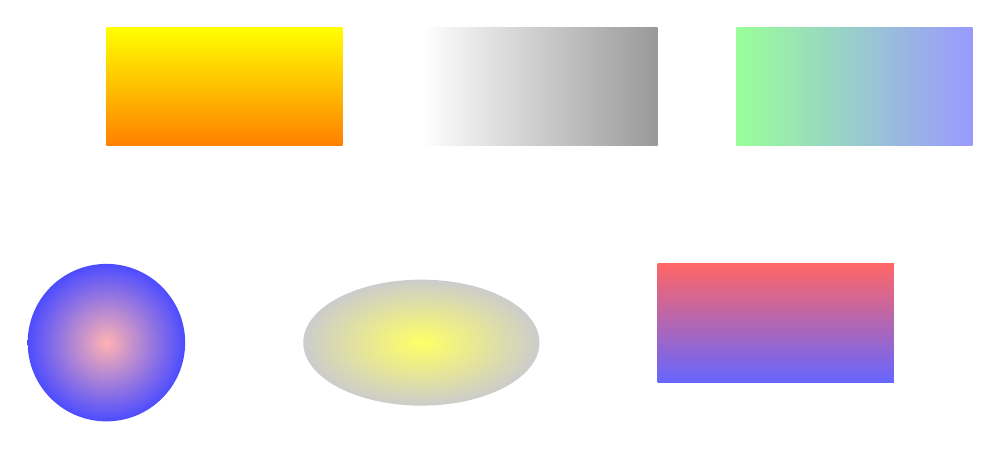
\begin{tikzpicture}
  % horizontal shading (top to bottom)
  \shade[top color=yellow, bottom color=orange] (0,0) rectangle (3,1.5);

  % tricolor shading
  \shade[left color=white, right color=black!40] (4,0) rectangle (7,1.5);

  % vertical + horizontal combo
  \shade[top color=green!40, bottom color=blue!40,
         left color=green!40, right color=blue!40]
    (8,0) rectangle (11,1.5);

  % inner color / outer color (radial-like axial)
  \shade[inner color=red!30, outer color=blue!70]
    (0,-2.5) circle (1);

  \shade[inner color=yellow!60, outer color=black!20]
    (4,-2.5) ellipse (1.5 and 0.8);

  % shading with opacity
  \shade[top color=red, bottom color=blue, opacity=0.6]
    (7,-3) rectangle (10,-1.5);
\end{tikzpicture}

\subsection*{Phase 13: Patterns and Decoration Extras}

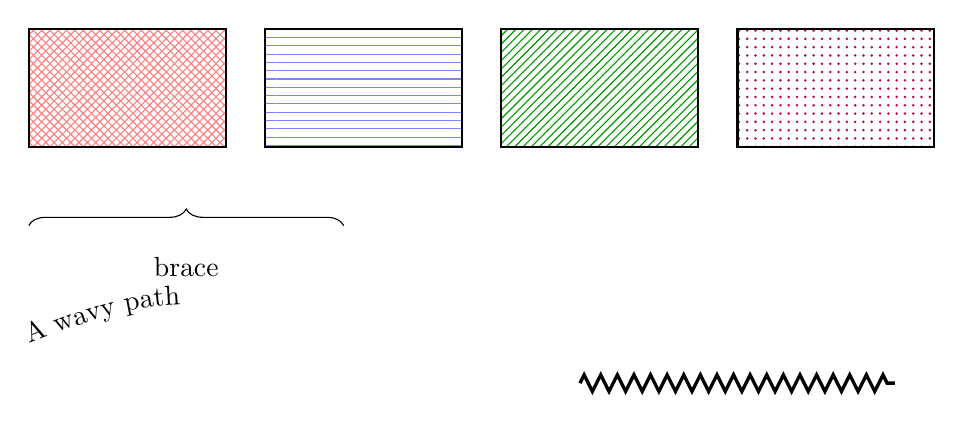
\begin{tikzpicture}
  % pattern fill (crosshatch)
  \fill[pattern=crosshatch, pattern color=red!50]
    (0,0) rectangle (2.5,1.5);
  \draw[thick] (0,0) rectangle (2.5,1.5);

  % pattern fill (horizontal lines)
  \fill[pattern=horizontal lines, pattern color=blue!50]
    (3,0) rectangle (5.5,1.5);
  \draw[thick] (3,0) rectangle (5.5,1.5);

  % pattern fill (north east lines)
  \fill[pattern=north east lines, pattern color=green!60!black]
    (6,0) rectangle (8.5,1.5);
  \draw[thick] (6,0) rectangle (8.5,1.5);

  % pattern fill (dots)
  \fill[pattern=dots, pattern color=purple]
    (9,0) rectangle (11.5,1.5);
  \draw[thick] (9,0) rectangle (11.5,1.5);

  % decoration: brace
  \draw[decorate, decoration={brace, amplitude=6pt}]
    (0,-1) -- (4,-1) node[midway, below=8pt] {brace};

  % decoration: text along path
  \draw[decorate, decoration={text along path,
        text={A wavy path}}] (0,-2.5) sin (2,-2) cos (4,-2.5) sin (6,-2);

  % more complex decoration
  \draw[very thick, decorate, decoration={
        zigzag, segment length=6pt, amplitude=3pt}]
    (7,-3) -- (11,-3);
\end{tikzpicture}

\subsection*{Phase 14: Advanced Path Connectors}

\begin{tikzpicture}
  % orthogonal connectors
  \node[draw] (A) at (0,0) {A};
  \node[draw] (B) at (2,1.5) {B};
  \draw[->] (A) |- (B);
  \draw[->] (A) -| (B);

  % various to-paths
  \node[draw] (C) at (5,0) {C};
  \node[draw] (D) at (8,1.5) {D};
  \draw[->, to path={-- (\tikztotarget)}] (C) -- (D);

  \node[draw] (E) at (5,-2) {E};
  \node[draw] (F) at (8,-0.5) {F};
  \draw[->] (E) to[out=60, in=180] (F);

  \node[draw] (G) at (5,-3.5) {G};
  \node[draw] (H) at (8,-3.5) {H};
  \draw[->] (G) to[bend left=45] (H);
  \draw[->] (H) to[bend left=45] (G);

  % edge with label
  \node[draw] (I) at (10,0) {I};
  \node[draw] (J) at (12,1) {J};
  \draw (I) edge[->, bend left] node[right] {label} (J);

  % loop
  \node[draw] (K) at (0,-3) {K};
  \draw[->] (K) edge[loop above] ();
  \draw[->] (K) edge[loop left] ();
\end{tikzpicture}

\subsection*{Phase 15: Node Anchor and Positioning}

\begin{tikzpicture}
  % named anchors
  \node[draw, shape=rectangle] (R) at (2,0)
    {\shortstack{anchor\\test}};
  \fill[red] (R.north) circle (1.5pt) node[above] {n};
  \fill[red] (R.south) circle (1.5pt) node[below] {s};
  \fill[red] (R.east)  circle (1.5pt) node[right] {e};
  \fill[red] (R.west)  circle (1.5pt) node[left] {w};
  \fill[red] (R.north east) circle (1.5pt);
  \fill[red] (R.north west) circle (1.5pt);
  \fill[red] (R.south east) circle (1.5pt);
  \fill[red] (R.south west) circle (1.5pt);

  % positioning with angles
  \node[draw] (S) at (7,0) {Source};
  \node[draw, above right=1cm and 0.5cm of S] {Above Right};
  \node[draw, below left=0.8cm and 0.3cm of S] {Below Left};

  % chain-like positioning
  \node[draw] (X0) at (2,-3.5) {X0};
  \node[draw, right=0.5cm of X0] (X1) {X1};
  \node[draw, right=0.5cm of X1] (X2) {X2};
  \draw[->] (X0) -- (X1) -- (X2);

  % above/below with offsets
  \node[draw] (P) at (8,-3) {P};
  \node[draw, above=0.3cm of P, xshift=8pt] {$Q_{up}$};
  \node[draw, below=0.5cm of P, xshift=-4pt] {$R_{dn}$};
\end{tikzpicture}

\subsection*{Phase 16: Foreach with Calculations}

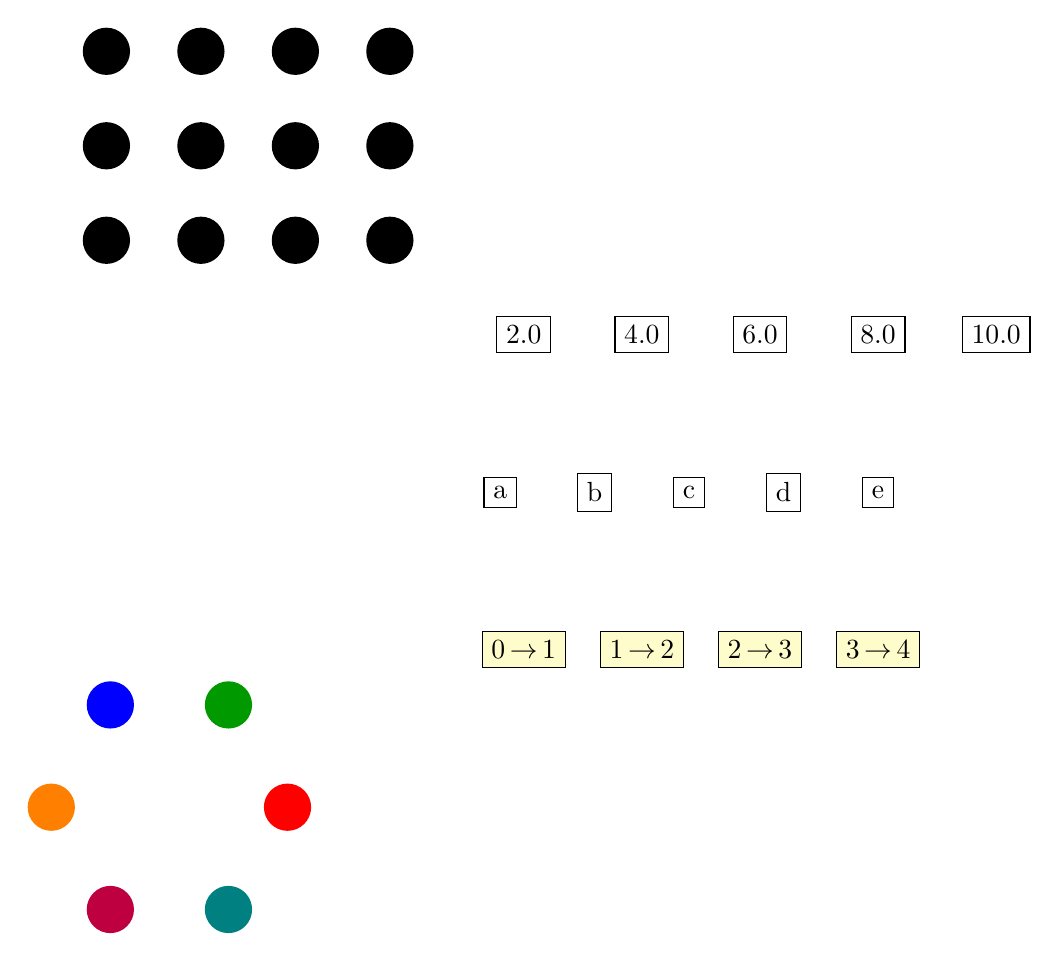
\begin{tikzpicture}
  % nested foreach
  \foreach \x in {1,...,4} {
    \foreach \y in {1,...,3} {
      \fill (\x*1.2, \y*1.2) circle (0.3);
    }
  }

  % foreach with evaluate
  \foreach \i [evaluate=\i as \j using \i*2] in {1,...,5} {
    \node[draw] at (\i*1.5+5, 0) {\j};
  }

  % count
  \foreach \x [count=\c] in {a,b,c,d,e} {
    \node[draw] at (\c*1.2+5, -2) {\x};
  }

  % remember
  \foreach \x [remember=\x as \lastx (initially 0)] in {1,...,4} {
    \node[draw, fill=yellow!20] at (\x*1.5+5, -4) {\lastx\,$\to$\,\x};
  }

  % foreach on named coordinates
  \coordinate (base) at (2,-6);
  \foreach \a/\r in {0/red, 60/green!60!black, 120/blue, 180/orange, 240/purple, 300/teal} {
    \fill[\r] ($(base) + (\a:1.5)$) circle (0.3);
  }
\end{tikzpicture}

\subsection*{Phase 17: Scopes with Style Inheritance}

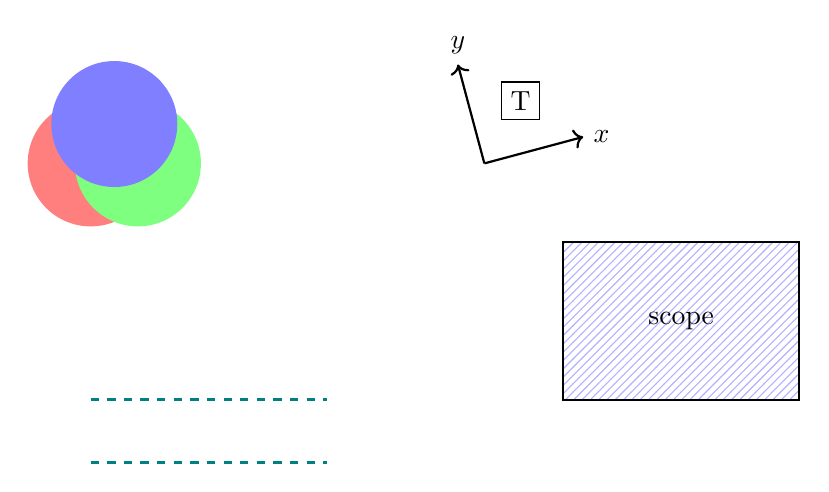
\begin{tikzpicture}
  % scoped opacity
  \begin{scope}[transparency group, opacity=0.5]
    \fill[red]   (0,0) circle (0.8);
    \fill[green] (0.6,0) circle (0.8);
    \fill[blue]  (0.3,0.5) circle (0.8);
  \end{scope}

  % scoped transform
  \begin{scope}[shift={(5,0)}, scale=1.3, rotate=15]
    \draw[thick, ->] (0,0) -- (1,0) node[right] {$x$};
    \draw[thick, ->] (0,0) -- (0,1) node[above] {$y$};
    \node[draw, fill=white] at (0.5,0.5) {T};
  \end{scope}

  % scoped line style
  \begin{scope}[very thick, color=teal, dashed]
    \draw (0,-3) -- (3,-3);
    \draw (0,-3.8) -- (3,-3.8);
  \end{scope}

  % scoped fill with pattern
  \begin{scope}[shift={(6,-2)}]
    \fill[pattern=north east lines, pattern color=blue!30]
      (0,-1) rectangle (3,1);
    \draw[thick] (0,-1) rectangle (3,1);
    \node at (1.5,0) {scope};
  \end{scope}
\end{tikzpicture}

\subsection*{Phase 18: Coordinate Calculations}

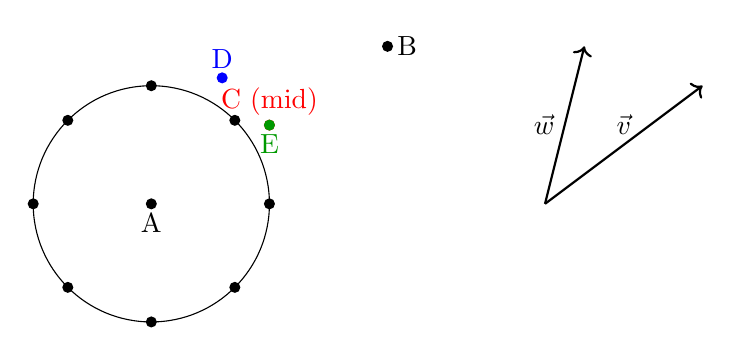
\begin{tikzpicture}
  % basic calculation
  \coordinate (A) at (0,0);
  \coordinate (B) at (3,2);
  \coordinate (C) at ($(A)!0.5!(B)$);
  \fill (A) circle (2pt) node[below] {A};
  \fill (B) circle (2pt) node[right] {B};
  \fill[red] (C) circle (2pt) node[above] {C (mid)};

  % point with offset
  \coordinate (D) at ($(A)!0.3!(B) + (0,1)$);
  \fill[blue] (D) circle (2pt) node[above] {D};

  % projection
  \coordinate (E) at ($(A)!(C)!(B)$);
  \fill[green!60!black] (E) circle (2pt) node[below] {E};

  % vector arithmetic
  \coordinate (V) at (5,0);
  \coordinate (W) at ($(V) + (2,1.5)$);
  \draw[->, thick] (5,0) -- (W) node[midway, above] {$\vec{v}$};
  \draw[->, thick] (5,0) -- ($(5,0) + (0.5,2)$)
    node[midway, left] {$\vec{w}$};

  % polar coordinates
  \foreach \angle in {0,45,...,315} {
    \fill (\angle:1.5) circle (2pt);
  }
  \draw (0,0) circle (1.5);
\end{tikzpicture}

\end{document}
